% Asset ID: AS2MeasuresLocationSpreadTikZ-005
% Purpose: Show variance and standard deviation.
\documentclass[tikz,border=8pt]{standalone}
\usepackage{amsmath}
\usetikzlibrary{arrows.meta, positioning, decorations.pathreplacing}
\begin{document}
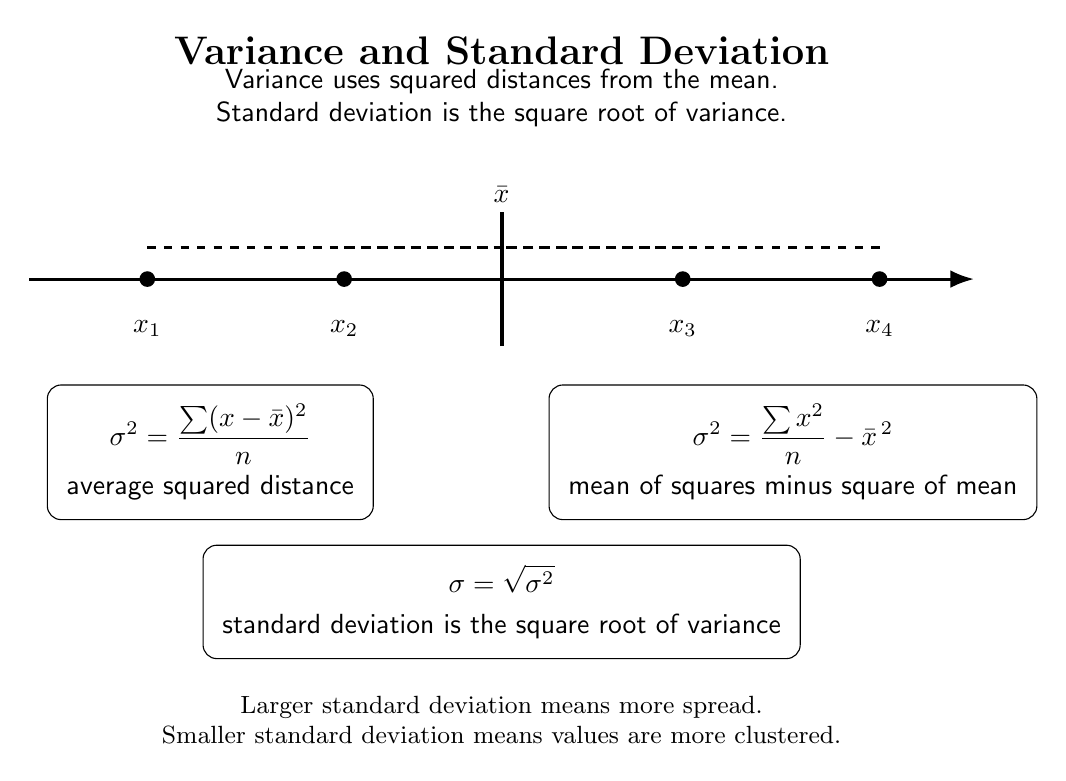
\begin{tikzpicture}[font=\sffamily, dot/.style={circle, fill=black, inner sep=2pt}, formula/.style={draw, rounded corners=5pt, align=center, inner sep=7pt}]
\node[font=\Large\bfseries] at (0,4.5) {Variance and Standard Deviation};
\node[align=center] at (0,3.9) {Variance uses squared distances from the mean.\\Standard deviation is the square root of variance.};
\draw[-{Latex[length=3mm]}, line width=1.1pt] (-6,1.6) -- (6,1.6);
\draw[line width=1.4pt] (0,0.75) -- (0,2.45);\node[above] at (0,2.45) {$\bar{x}$};
\foreach \x/\name in {-4.5/x_1, -2.0/x_2, 2.3/x_3, 4.8/x_4}{\node[dot] at (\x,1.6) {};\node[below=4mm] at (\x,1.6) {$\name$};\draw[dashed, thick] (\x,2.0) -- (0,2.0);}
\node[formula] at (-3.7,-0.6) {$\displaystyle \sigma^2=\frac{\sum (x-\bar{x})^2}{n}$\\[3pt]average squared distance};
\node[formula] at (3.7,-0.6) {$\displaystyle \sigma^2=\frac{\sum x^2}{n}-\bar{x}^{\,2}$\\[3pt]mean of squares minus square of mean};
\node[formula] at (0,-2.5) {$\displaystyle \sigma=\sqrt{\sigma^2}$\\[3pt]standard deviation is the square root of variance};
\node[align=center, font=\small] at (0,-4.0) {Larger standard deviation means more spread.\\Smaller standard deviation means values are more clustered.};
\end{tikzpicture}
\end{document}
